\documentclass{paper}
\usepackage[margin=0.5in]{geometry}
\usepackage{graphicx}
\title{3. Busser}
\begin{document}
\maketitle
\begin{large}\textbf{Hvad er en bus?}\end{large}

\line(1,0){510}
\begin{itemize}
	\item En forbindelse mellem komponenter
	\item B\aa de interne og eksterne
	\begin{itemize}
		\item \textbf{Internt mellem system komponenter}
		\begin{itemize}
						\item SPI, I$^{2}$C - Seriel
		\end{itemize}
		\item \textbf{Eksterne komponenter}
		\begin{itemize}
			\item eSATA
			\item USB(Universal Serial Bus)
		\end{itemize}
	\end{itemize}	
	\item Kan ogs\aa\ benyttes internt i en chip
	\begin{itemize}
		\item Mange paralelle forbindelser kan indg\aa\
		\item H\o j b\aa ndbredde
		\item F.eks. internt i en CPU
	\end{itemize}
	\item Busser bliver ofte delt mellem flere komponenter, med kun en CPU er delte busser lige s\aa\ effektive som seperate busser
\end{itemize}

\begin{large}\textbf{Hvilke signaler benytter man typisk p\aa\ en parallel bus?}\end{large}

\line(1,0){510}
\begin{itemize}
	\item P\aa\ en typisk microprocessor:
	\begin{itemize}
		\item Select Address on slave device
		\item Data to/from slave device
		\item Select, read, write and wait signals
		\item Slave interrupts
		\item Multi-master Control signals(Daisy Chaining, device t\ae ttest p\aa\ f\aa r adgang f\o rst
		\item Special Handshaking signals
		\item Misc. signals	
	\end{itemize}
\end{itemize}

\begin{large}\textbf{Hvordan adresserer man p\aa\ en bus?}\end{large}

\line(1,0){510}
\begin{itemize}
	\item Der benyttes en adresse bus
	\item For at kunne adressere 64K (2$^{16}$) memory, skal der benyttes 16 adresse linjer  
	\item READ/ fra host, er forbundet til OE/(output enable) p\aa\ modtageren
	\item WRITE/ til WE/(write enable)
	\item Hosten ved reelt ikke hvad der sidder p\aa\ hvilke adresser
	\begin{itemize}
		\item Derfor vil "address spaces" som regel v\ae re delt op til hver enhed
		\item F.eks. en opdeleing mellem RAM - mest betydende bit altid 0, og ROM - mest betydende bit altid 1
	\end{itemize}
	\item (Byte-enable(NBE0, NBE1) kan benyttes til at l\ae se en halv atomic memory block) 
\end{itemize}

\begin{large}\textbf{Hvilke ting skal konfigureres p\aa\ en host for at kunne tale med et device p\aa\ en bus?}\end{large}

\line(1,0){510}
\begin{itemize}
	\item Adresse
	\begin{itemize}
		\item Adressen p\aa\ bussen
		\item Chipselect til den specifikke enhed p\aa\ bussen
	\end{itemize}
	\item Read/Write - host skal vide om der \o nskes at l\ae se fra eller skrive til devicen
	\item Timing, Clockhastigheden skal v\ae re den samme p\aa\ host og device
\end{itemize}

\begin{large}\textbf{Beskriv et l\ae se/skrive scenarie og de timing parametre som indg\aa r}\end{large}

\line(1,0){510}
\begin{itemize}
	\item Wait states til langsomme eksterne enheder
\end{itemize}

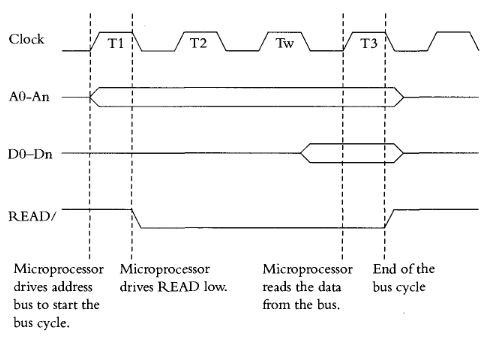
\includegraphics[scale=0.7]{busreadwaitstate.png}
	
\textit{Note: Der kan v\ae re et wait signal sendt fra devicet til CPU'en}

\end{document}
